%% ------------------------------------------------------------------------- %%
\chapter{Protótipo e Ferramentas Selecionadas}
\label{cap:prototype}

%A partir da arquitetura apresentada no \autoref{cap:arquitetura}, um protótipo do sistema CEP Handler foi construído. 


%TROCAR FOOTNOTES POR CITAÇÔES

%Neste capítulo é apresentado o protótipo de implementação da arquitetura de microsserviços vista no \autoref{cap:arquitetura}. São apresentadas as ferramentas utilizadas para o desenvolvimento de cada parte, além de uma justificativa para escolha de cada uma.

%------------------------------------------------------
%\section{Ferramentas selecionadas} 

Neste trabalho, um protótipo da arquitetura para sistema de CEP distribuído apresentada no Capítulo~\ref{cap:arquitetura} foi implementado e avaliado. 
A escolha das ferramentas para a implementação do protótipo levou em conta vários fatores que dependem da função de cada ferramenta no sistema. Mas um dos critérios de seleção que foi aplicado em todos os casos foi o de que todo o software utilizado na implementação deveria ser de \textit{software} livre, com uma licença que garantisse a visualização,  alteração e distribuição do código da ferramenta. O código desenvolvido pode ser encontrado no repositório online GitLab~\citep{CEPHandler}, a \autoref{fig:system_architecture_prto} representa a arquitetura do sistema com as ferramentas selecionadas.
As seções a seguir apresentam detalhes sobre a escolha das ferramentas e a implementação do protótipo.


\begin{figure}[hb!]
      \centering
      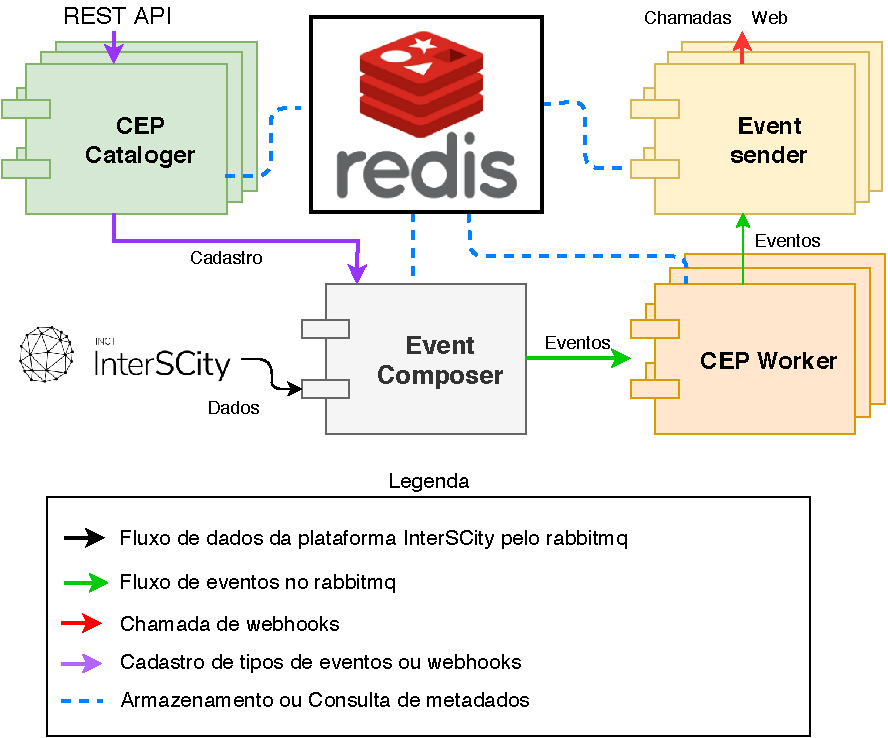
\includegraphics[width=0.8\textwidth]{figuras/graphics/prot_dia.pdf}
      \caption{Protótipo da arquitetura do \texttt{CEP Handler}}
      \label{fig:system_architecture_prto}
\end{figure}

%\todo[inline]{Fernando, você poderia criar uma nova versão da imagem da sua arquitetura com os nomes das ferramentas usadas em cada microsserviço, para dar uma visão geral da escolhas de implementação.  Essa imagem poderia ficar aqui, na introdução do capítulo 5.}

\subsubsection{A Plataforma InterSCity}
A plataforma de cidades inteligentes InterSCity, projetada e desenvolvida pelo Instituto Nacional de Ciência e Tecnologia da Internet do Futuro para Cidades Inteligentes~\citep{del2019design}, sediado no IME-USP, para o desenvolvimento e suporte a projetos de Cidades Inteligentes. O principal propósito da plataforma é prover serviços de alto nível e APIs RESTful para suporte no desenvolvimento de novos serviços para as cidades. A plataforma adota uma arquitetura de microsserviços para suportar a integração de uma grande quantidade de recursos e dados e prover serviços de qualidade para a cidade. Os sensores ou atuadores na cidade são considerados Recursos, que podem enviar diferentes tipos de dados. Cada Recurso está associado a uma ou mais Capacidades, que descrevem quais tipos de dados os sensores podem coletar ou quais ações os atuadores podem realizar. A seguir, são descritos os principais microsserviços da plataforma:

%serve para unificar os vários serviços urbanos, de forma que possam interagir mais facilmente e que exista uma maior interação entre diversos setores da administração pública, entre entidades governamentais e serviços privados e entre todas as partes envolvidas\todo{Essa descrição da plataforma está muito baseada em "interação" entre serviços e órgãos, parece muito idealizada. Aqui, é melhor você apresentar uma definição mais tecnológica dela, como a que aparece em https://interscity.org/software/interscity-platform/ }. Ela consiste em um conjunto de microsserviços, no qual cada um tem uma função diferente relacionada ao manuseio de dados urbanos.

\begin{itemize}
\item \textbf{Resource Adaptor}: responsável por coletar dados enviados em tempo real por sensores espalhados pela cidade.
\item \textbf{Actuator Controller}: responsável por enviar comandos para atuadores na cidade.
\item \textbf{Resource Cataloger}: responsável por manter um registro de todos os sensores e atuadores na cidade, além dos tipos de Capacidades que cada Recurso possui e do esquema dos dados que cada Capacidade envia.
\item \textbf{Data-Collector}: responsável por manter uma cópia de todos os dados coletados para análises em lotes.
\item \textbf{Resource-Viewer}: responsável por fazer a interação da plataforma com usuários por interface gráfica.
\end{itemize}

A plataforma InterSCity possibilita o cadastro de novos Recursos e Capacidades por uma API RESTful, além da visualização dos dados já coletados. O microsserviço \texttt{Event Composer} da ferramenta \texttt{CEP Handler}, descrito na Seção \ref{sec:eventcomposer}, se conecta com o Resource Adaptor, para receber os dados em tempo real, e com o Resource Cataloger, para saber o esquema dos dados recebidos e convertê-los em eventos. Todos os dados enviados em tempo real para o sistema podem ser convertidos em eventos e ser utilizados na definição de outros eventos.
Como o sistema de processamento de eventos desenvolvido neste trabalho foi implementado acoplado à plataforma do InterSCity, escolheu-se um nome em inglês para ele (\texttt{CEP Handler}), para manter o mesmo estilo de nomenclatura já usado nos microsserviços da plataforma.  


\section{Ferramenta de Processamento de Eventos}
Para o processamento de eventos nos nós do sistema distribuído (ou seja, nas instâncias de \texttt{CEP Worker}), foi escolhida a ferramenta mais utilizada pela comunidade de CEP e que possui a interface mais conhecida -- a \cite{ESPER}. As vastas documentação e comunidade de apoio dessa ferramenta facilitaram o seu uso na implementação do sistema \texttt{CEP Handler} e a comparação de seu desempenho com o de outros trabalhos relacionados, visto que muitos deles também utilizaram ESPER como ferramenta de CEP.

%\subsection{Representação de Eventos}

A ESPER permite representar eventos em alguns formatos diferentes, porém somente três deles apresentam bom desempenho\citep{EsperEventRepresentation}:

\begin{itemize}
\item \textbf{Java Object Array}: possibilita trabalhar com eventos representados por vetores de objetos, em que cada campo do objeto representa um campo do evento. Essa abordagem permite trabalhar com qualquer evento, mesmo quando não se sabe quais medidas ou campos ele contém, mas tem a desvantagem de ser uma representação específica da linguagem Java.
\item \textbf{Classe Java - POJO}: possibilita representar cada evento como uma definição de classe em um arquivo Java. Esse formato só pode ser utilizado para tratar eventos em um contexto no qual os campos já são previamente conhecidos, o que não condiz com a proposta deste trabalho, ou utilizando geração automática de código Java, o que tornaria necessário recompilar o \texttt{CEP Worker} e instanciá-lo novamente toda vez que um novo evento fosse cadastrado em uma instância dele ativa, forçando o sistema a parar o processamento para isso.
\item \textbf{Apache Avro}: Apache \cite{Avro} é um protocolo de seriação de dados implementado em várias linguagens. Ele apresenta um desempenho interno tão bom quanto um vetor de objetos Java, com a vantagem de poder ser lido por outros softwares em outras linguagens. Feito inicialmente para o Apache \cite{hadoop}, atualmente ele é aceito em vários sistemas de processamento em tempo real além do ESPER, como Apache \cite{spark}, o que diminui o custo de integração com outros serviços no futuro.
\end{itemize}

Foi escolhido o uso de Apache Avro para a representação de enventos neste trabalho, por ser independente do Java, desta forma deixando o sistema mais desacoplado de qualquer linguagem de programação. 

%\todo[inline]{Ué, a seção termina sem explicar qual desses formatos é de fato usado no seu sistema. }

\section{Microsserviços sem Estado}
O \textit{CEP Cataloger}, Event Composer e Event Sender são microsserviços que só oferecem métodos que não guardam estado. A implementação dos três microsserviços foi feita usando Docker para o isolamento de ambiente de execução, de forma que poderiam ser escritas em qualquer linguagem de programação com suporte a clientes dos outros serviços. Pelo conhecimento prévio em Java, essa foi a linguagem escolhida para o desenvolvimento dos três microsserviços.


%utilizando a ferramenta de automação\todo{automação de que?} \cite{maven} para inserção de dependências e colocados dentro de imagens Docker\todo{Rever o final da frase, há um erro de concordância que está comprometendo a compreensão.}.
%\todo[inline]{Na Seção 2.2, você explica o que é contêiner, mas não fala nada sobre imagens. Como aparece aqui, é bom definir lá também o que é uma imagem e qual a relação dela com contêiner.}

%\section{Isolamento de Ambientes Virtuais}
%Como discutido na Seção \ref{sec:cloudtools}, a utilização de contêineres facilita a execução de sistemas com arquiteturas de microsserviços. Atualmente, a ferramenta \cite{Docker} é o padrão \textit{de facto} para conteinerização, é a mais utilizada pela comunidade. A empresa que desenvolve a Docker mantém um repositório de imagens, o \cite{dockerhub}, onde são mantidas as imagens oficiais de programas que podem ser conteinerizados. Estes repositórios são feitos pela própria empresa Docker ou pela comunidade que administra cada uma das ferramentas, além de permitir que usuários comuns armazenem suas próprias imagens\todo{Essa última frase está confusa. Ela fala de "repositórios de ferramentas", mas a anterior fala de "imagens de programas" mantidas em só repositório. É bom rever e esclarecer.}.

%\todo[inline]{Nesta seção, você fala sobre o docker e o repositório de imagens que ele mantém, mas  termina sem explicar como eles foram usados na implementação que você fez. :(  }


%Para que os microsserviços fiquem em ambientes isolados, recomenda-se utilizar uma ferramenta que ofereça virtualização no nível do sistema operacional, normalmente conhecida como conteinerização. Há duas principais vantagens em se usar contêineres para implementar uma aplicação: o fato de a aplicação feita em contêiner ter suas dependências mantidas dentro do contêiner garante que ela poderá ser executada em qualquer outra máquina e, em contraste com Máquinas Virtuais que emulam o hardware, os contêineres somente virtualizam o sistema operacional, em geral utilizando menos recursos.
\section{Orquestração de Contêineres}

Para executar os contêineres em ambientes de nuvem, existem várias alternativas, entre elas: executá-los diretamente em máquinas virtuais, utilizar orquestradores de contêineres proprietários, como o \textit{Elastic Container Service} - \cite{awsecs} da AWS, ou utilizar orquestradores de \textit{software} livre.



Entre os orquestradores de \textit{software} livre, três se destacam:

\begin{itemize}
    \item \textbf{Apache Mesos}~\citep{Mesos}: Desenvolvido inicialmente pela universidade de Berkeley, depois passou a ser mantido pela Apache Foundation. Foi desenvolvido sem foco em contêineres, mas em coordenação de \textit{clusters} de computadores.
    \item \textbf{Docker Swarm}~\cite{Swarm}: Desenvolvido pela mesma empresa que mantém a ferramenta Docker, o Docker Swarm tem compatibilidade nativa com o sistema de isolamento de ambientes Docker.
    \item \textbf{Kubernetes}~\citep{Kubernetes}: Desenvolvido pela Google com o codinome Borg internamente, teve seu \textit{software} livre e passou a ser mantido pela \textit{Cloud Native Computing Foundation} - \cite{cnfc}. A CNCF é uma fundação voltada ao desenvolvimento de ferramentas para sistemas feitos nativamente para execução em nuvem.
\end{itemize}  
    
\cite{Truyen_2019} fizeram uma comparação dos três orquestradores de contêineres e concluíram que o Kubernetes oferece o maior número de opções de configuração entre os três. Além disso, é o único que possui suporte nativo pelas três maiores provedoras de computação em nuvem (AWS, GCP e Azure). Por esses motivos, o Kubernetes foi escolhido para a implementação do protótipo aqui apresentado.


\section{Transmissão Assíncrona}

Para a transmissão de eventos em tempo real foi escolhido o \textit{broker} de mensagens RabbitMQ~\citep{RabbitMq}. RabbitMQ é um dos mais usados brokers atualmente, pois suporta vários protocolos de comunicação assíncrona~\citep{Dobbelaere:2017:KVR:3093742.3093908}. O principal fator para a escolha do RabbitMQ como \textit{broker} foi a compatibilidade com a plataforma InterSCity, cuja implementação já utiliza o RabbitMQ como mensageiro assíncrono. Já que o sistema proposto neste trabalho foi desenvolvido como uma extensão da plataforma InterSCity, é interessante utilizar em sua implementação as mesmas ferramentas usadas na plataforma, para permitir uma maior integração entre eles.
No protótipo do sistema aqui apresentado, o RabbitMQ opera dentro de um contêiner Docker, cuja imagem é disponibilizada oficialmente pelo repositório de imagens Docker Hub. 



%Vários \textit{brokers} são utilizados atualmente, com vários protocolos diferentes. Dois que se destacam entre os muitos são o Apache \cite{Kafka} e o \cite{RabbitMq}. Uma comparação extensa entre as duas ferramentas foi feita por \cite{Dobbelaere:2017:KVR:3093742.3093908}.

%\subsubsection{Apache Kafka}
%Baseado em um sistema de análise de \textit{logs}, o Apache Kafka utiliza um sistema próprio para transmissão de mensagens de forma assíncrona\todo{Mas quais são as características desse sistema? O que ele tem de interessante, o que faz ele ser um dos mais usados? Esses mesmos comentários valem para a explicação que você deu sobre o RabbitMQ}.
%Ele é o mensageiro padrão para entrada e saída de mensagens na maioria dos sistemas de processamento de Big Data em tempo real, como Apache \cite{Storm} e Apache \cite{spark}.

%\subsubsection{RabbitMQ}
%O Rabbitmq é um transmissor de mensagens assíncronas que utiliza uma versão modificada do protocolo AMQP\todo{o que significa a sigla?}. Atualmente, é o mensageiro assíncrono mais utilizado para diferentes tipos de sistemas\todo{Antes, vc disse que o Kafka é o padrão na maioria dos sistemas de processamento em tempo real. Qual das afirmações é a verdadeira?}. 


%Neste trabalho, decidiu-se pelo uso do RabbitMQ por dois motivos principais:
%\begin{itemize}
%\item O Kafka não permite a exclusão de tópicos. Cada tópico de transmissão de mensagens criado funciona como uma fila de mensagens para o consumidor, sendo permanente, e o Kafka não permite eliminar tópicos que deixaram de ser utilizados. Como o sistema distribuído proposto neste trabalho tem topologia dinâmica, isso seria uma sobrecarga desnecessária ao sistema.%\todo{"má prática" não parece a justificativa correta aqui. Os tópicos "inativos" não seriam uma sobrecarga desnecessária ao sistema?}.
%\item A plataforma InterSCity já utiliza o RabbitMQ como mensageiro assíncrono. Já que o sistema proposto neste trabalho foi desenvolvido como um serviço da plataforma InterSCity, é interessante utilizar em sua implementação as mesmas ferramentas usadas na plataforma, para permitir uma maior integração entre eles.
%\end{itemize}




\section{Sistema Gerenciador de Banco de Dados}
Como sistema gerenciador de banco de dados, para guardar a definição dos eventos e seus metadados, foi escolhido o \cite{Redis}, um sistema \textit{NoSQL} baseado no modelo de dados chave-valor.
O Redis foi escolhido por ser de \textit{software} livre, ter uma grande comunidade de usuários e apresentar uma das menores latências entre sistemas gerenciadores de bancos de dados~\citep{10.14778/2367502.2367512}.
No protótipo do sistema \texttt{CEP Handler} desenvolvido, o Redis opera dentro de um único contêiner Docker, cuja imagem é disponibilizada oficialmente pelo repositório de imagens \textit{Docker Hub}.
 

Para o armazenamento chave-valor, são usados como chaves para os tipos de eventos identificadores do tipo UUID - (\textit{universally unique identifier}). A unicidade deste tipo de identificador não depende de um registro central ou de coordenação entre diferentes partes do sistema distribuído para poderem garantir sua unicidade, em contraste com a maioria dos identificadores. A probabilidade que um UUID seja duplicado é negligenciável. O método para a geração desse tipo de identificador é reconhecido pela Open Software Foundation
\citep{osf}, 
%(OSF)\footnote{\url{https://pubs.opengroup.org/onlinepubs/9629399/apdxa.htm}},
pela  Internet Engineering Task Force %(IETF)\footnote{\url{https://tools.ietf.org/html/rfc4122}}
\citep{ietf}
e como parte do  ISO/IEC 11578:1996 "Information technology – Open Systems Interconnection – Remote Procedure Call (RPC)" e mais recentemente em  ITU-T Rec. X.667 | ISO/IEC 9834-8:2005
%\footnote{\url{https://www.itu.int/ITU-T/studygroups/com17/oid.html}}
\citep{ISOUUID}.%\todo{Revisar esse trecho final bagunçado. Vc queria dizer que o UUID é "reconhecido" ou "recomendado"? - reconhecido.}

No sistema \textit{CEP Handler}, associados a  uma chave UUID de tipo de evento estão: os tipos de eventos que lhe servem de entrada, o nome do tipo de evento, a sua definição em EPL e os endereços de \textit{Web Hooks} a serem chamados no caso da detecção de eventos desse tipo.


%\todo[inline]{Incluir no início da capítulo a URL do repositório da sua implementação.}
